
\documentclass[12pt]{article}
\usepackage{graphicx}
\usepackage{amsmath}
\usepackage{mathtools}
\usepackage{gensymb}
\usepackage{amssymb}

\newcommand{\mydet}[1]{\ensuremath{\begin{vmatrix}#1\end{vmatrix}}}
\providecommand{\brak}[1]{\ensuremath{\left(#1\right)}}
\providecommand{\norm}[1]{\left\lVert#1\right\rVert}
\newcommand{\solution}{\noindent \textbf{Solution: }}
\newcommand{\myvec}[1]{\ensuremath{\begin{pmatrix}#1\end{pmatrix}}}
\providecommand{\abs}[1]{\left\vert#1\right\vert}	
\let\vec\mathbf

\begin{document}
\begin{center}
\textbf\large{CLASS 11 CHAPTER-11 \\ LINES}

\end{center}
\section*{Exercise 10.3}

Q5.Find the points on the x-axis, whose distances from the line $\frac{x}{3}+\frac{y}{4}=1$ are 4 units.

\solution
Given line is 
\begin{align}
	\frac{x}{3}+\frac{y}{4}=1
\end{align}
which can be written as
\begin{align}
	4x+3y=12
\end{align}
this equation can be expressed as 
\begin{align}
	\vec{n}^{\top}\vec{x}=c
\end{align}
\begin{align}
	\text{ where }
		\vec{n} = \myvec{4\\3} , c = 12
\end{align}
Now we know the distance formula is given as
\begin{align}
	d = \frac{\abs{\vec{n}^\top\vec{P}-c}}{\norm{\vec{n}}}
\end{align}
Since it is given that point lies on the x-axis so let
\begin{align}
	\vec{P} = x\vec{e}_{1} = \myvec{x\\0}
\end{align}
Substituting the values in the given formula we get
\begin{align}
	d &= \frac{\abs{\vec{n}^\top\vec{P}-c}}{\norm{\vec{n}}}\\
	  &= \frac{\abs{x\vec{n}^\top\vec{e}_{1}-c}}{\norm{\vec{n}}}
\end{align}
So,
\begin{align}
	\abs{x\vec{n}^\top\vec{e}_{1}-c} &= d\norm{\vec{n}}
\end{align}
So, either
\begin{align}
	x = \frac{d\norm{\vec{n}}+c}{\vec{n}^\top\vec{e}_{1}}
\end{align}
Or,
\begin{align}
	x = \frac{-d\norm{\vec{n}}+c}{\vec{n}^\top\vec{e}_{1}}
\end{align}
where,
\begin{align}
	\vec{n} &= \myvec{4\\3}\\
	\norm{\vec{n}} &= \sqrt{4^2+3^2} = 5\\
	d &= 4\\
	c &= 12\\
	\vec{e}_{1} &= \myvec{1\\0}
\end{align}
So, substituting the values we get either
\begin{align}
	x = 8
	\text{ Or }
	x = -2
\end{align}
Hence, the two points that satisfy the above criteria are $\myvec{-2\\0} \text{ and } \myvec{8\\0}$ as shown in Figure \ref{fig:Fig1}	

\begin{figure}[!h]
	\begin{center} 
	    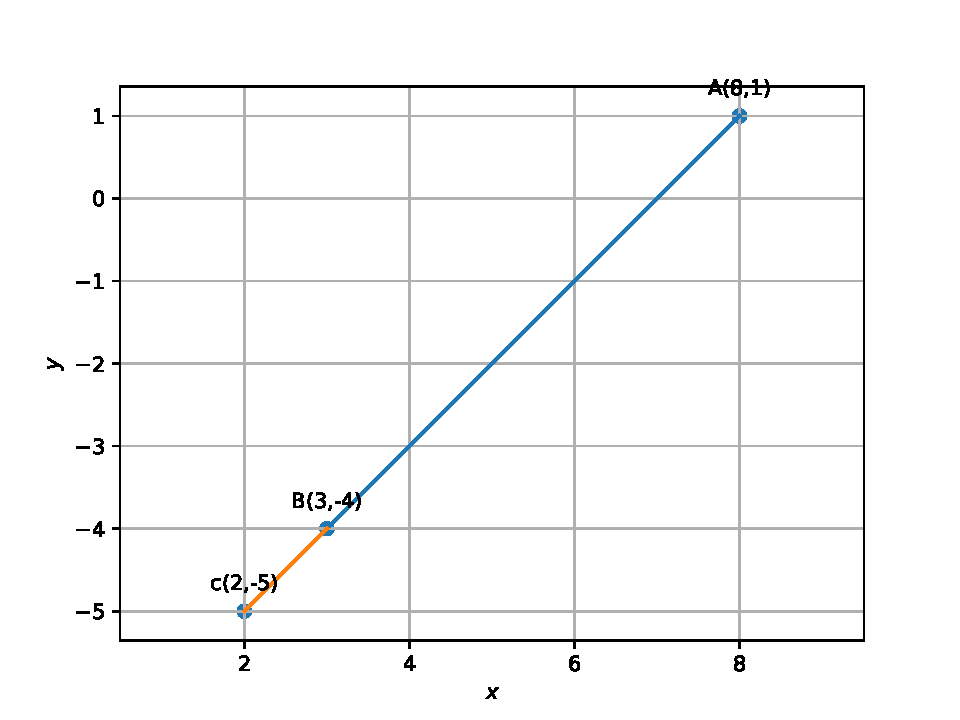
\includegraphics[width=\columnwidth]{figs/line2}
	\end{center}
\caption{}
\label{fig:Fig1}
\end{figure}

\end{document}

